% \documentclass{article}

% % Language setting
% % Replace `english' with e.g. `spanish' to change the document language
% \usepackage[english]{babel}

% % Set page size and margins
% % Replace `letterpaper' with `a4paper' for UK/EU standard size
% \usepackage[letterpaper,top=2cm,bottom=2cm,left=3cm,right=3cm,marginparwidth=1.75cm]{geometry}

% % Useful packages
% \usepackage{amsmath}
% \usepackage{graphicx}
% \usepackage[colorlinks=true, allcolors=blue]{hyperref}

\documentclass[12pt]{article}
\usepackage{graphicx}
\usepackage[utf8]{inputenc}
\usepackage{makecell}
\usepackage[margin=0.7in]{geometry}
\usepackage[T1]{fontenc}
\usepackage{mathptmx}
\usepackage[normalem]{ulem}
\usepackage{url}
 \usepackage{float}
\usepackage{hyperref}
\renewcommand\theadalign{bc}
\renewcommand\theadfont{\bfseries}
\renewcommand\theadgape{\Gape[4pt]}
\renewcommand\cellgape{\Gape[4pt]}

\usepackage[
backend=biber,
style=numeric,
sorting=ynt
]{biblatex}

\addbibresource{References.bib}
% \bibliography{mybib}
% \bibliographystyle{chem-rsc}


% openning
\title{\textbf{Semi automated squash refereeing system using computer vision and machine learnings}}
\author{Ahmed Said,  Hussein Amr, Seif Nasser, Youssef Mohamed ْ\\
Supervised by: Dr. Taraggy Ghanim }

\begin{document}
\maketitle
\begin{table}[H]
\begin{tabular}{|l|l|l|}
\hline
\thead{Proposal Version}    & \thead{Date} & \thead{Reason for Change}  \\ \hline
1.0 & 24-October-2023   & \makecell{Proposal First version’s specifications are defined}   \\ \hline
2.0 & 14-November-2023   & \makecell{Proposal Challenges , Contribution, Time Line}\\ \hline
\end{tabular}
\caption{Document version history}
\end{table}

\textbf{GitHub: }\href{https://github.com/sa3eed-x/semi-automated-squash-refereeing-system}{semi-automated-squash-refereeing-system}

\begin{abstract}

With 20 million players worldwide in over 185 countries, squash is considered one of the most famous sports in the world. In the dynamic and fast-paced world of squash, the need for an advanced refereeing system has emerged as more and more evident so as to reduce the human error as time passes.Our project aims to help fulfill this need by developing and implementing a functional squash system that is ready to transform the game of squash through artificial intelligence. Unlike traditional structures
that rely completely on human sources, our answer harnesses modern computer vision like YOLO and openCV , data analytics and machine learning like SVM and RNN and use these technologies to autonomously and accurately officiate in real-time. In the end, this system hopes to ensure fair and consistent decisions and improve the overall squash experience for players and fans.In addition, it tries to revolutionize playing and watching squash by addressing the needs and expectations of players, referees, fans, and investors, thereby making squash a game that embraces technological innovation.
\end{abstract}

\section{Introduction}

\subsection{Background}

Squash is a sport loved by a huge number of athletes in many countries worldwide, holding a prominent place as one of the most globally cherished athletic activities. The high-paced nature of the game poses obstacles to precise decision-making in refereeing, and the inherent subjectivity in human judgment can occasionally result in disagreements among players. players start a rally by taking turns hitting the ball the ball must be hit above the tin and below the out line on the front wall. The player wins a point when the receiver fails to hit the ball before it bounces twice. or commits a foul which is called a “Stroke”. A stroke decision is taken by the referee, he may also call for a Let or No Let based on his POV. Additionally, according to world squash officiating \cite{world-squash-officiating} in some cases, a small human failure, like the referee making the wrong decision during a match, could be the reason for changing the whole world ranking in an unfair way. And because refereeing is an important factor in squash, as in any other kind of sport, using today’s technology is a significant gain for the world, benefiting efforts to solve this issue. Consequently, the necessity for an innovative refereeing system becomes ever more evident, striving to elevate precision, equity, and the overall enjoyment of squash.
\subsection{Motivation}

\subsubsection{Academic}
The fact behind this project's academic drive emerges from the acknowledgement of an existing void within the realm of research pertaining to squash refereeing systems. While numerous sports have used the rewards of technological progress, squash has yet to fully exploit the capabilities of computer vision and machine learning in its officiating procedures. The primary objective of this project is to narrow this gap by introducing groundbreaking solutions, thereby making a valuable contribution to the scholarly conversation surrounding sports technology and the utilization of artificial intelligence in squash.

\subsubsection{Business}
The main business behind this project centers on fulfilling the refereeing requirements of the squash community and industry. By introducing a semi-automated squash refereeing system, the project aligns with market demands for equitable competition, minimized errors, and an elevated viewing experience. In addition to catering to the needs of players and fans, the system possesses the potential to attract investments, positioning itself as a pioneering technology within the sports industry. The ultimate goal of this project is to meet the expectations of players, referees, fans, and investors alike, establishing squash as a leading force in embracing technological innovation. especially since squash was added to the 2028 Olympics, and everyone who supports squash needs this event to be in perfect shape.

\subsection{Problem Statement}
Manual refereeing in squash is prone to human error and subjectivity, leading to inaccurate decisions. The fast-paced nature of the game can cause difficulties in accurately tracking players' movements and the ball, resulting in missed calls or incorrect judgments. Personal biases and differing interpretations of rules can further inaccuracies, causing frustration and disputes among players.
\cite{TechAndHuman}\\\\
Defining a ball's out of bounds, identifying fouls or interference, and accurately awarding points are also challenging for the referee.\\\\
Referees must maintain control and ensure fair play in an intense, competitive sport, despite potential unsportsmanlike behavior. This can create frustration and impact the fairness and integrity of the game.\\

\section{Project Description}
\begin{figure}[H]
    \centering
    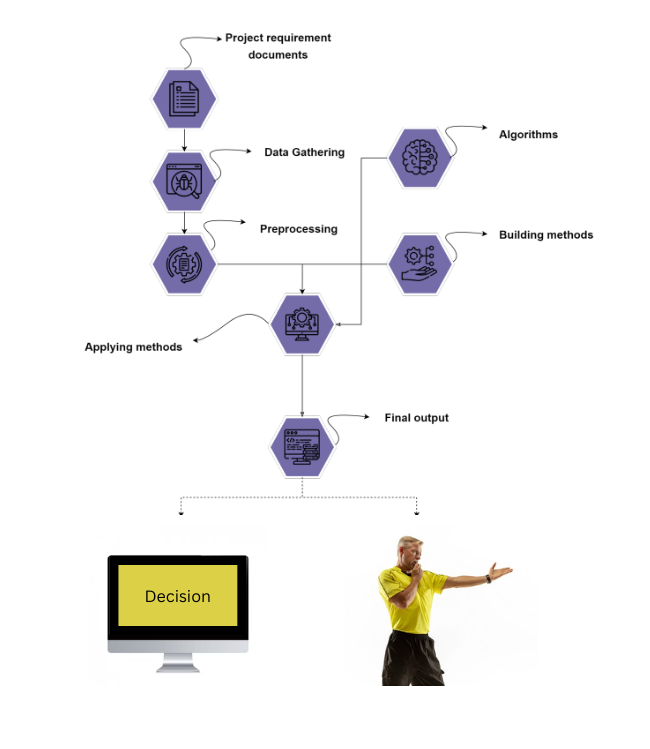
\includegraphics[width=0.75\linewidth]{figures/Project description.png}
    \caption{Project description}
    \label{fig:Project description}
\end{figure}

’Figure 1’ illustrate our project flow. we begin by getting data from live match broadcasts , preprocess it And then we apply algorithms based on the required output and
the best performance given.We prepare all this data to be ready to apply the methods. Then the output is given as an autonomous decision or semi-autonomous by giving the referee the choice to choose based on the system voting.

\subsection{objective}
This project is meant to make the squash refereeing process unbiased and more accurate while reducing human error as much as possible. The system objective is to design, develop, and implement a solution that detect and track the players and ball throughout a live squash match and Make highly accurate decisions based on squash rules violations and help the referee in taking the critical foul decisions.To achieve this, the system will require proper gathering and creation of our own Data set of specifications of the fouls( Let, No Let, Stroke), Machine learning, and Deep learning.


\begin{itemize}
    \item  The system will enhance the overall refereeing experience and contribute to fair play in the sport of squash.
    \item The system will detect the players and ball by computer vision algorithms and track them with the suitable deep learning techniques.
    \item The system will use machine learning which provides it with foul detection and gives the referee the right decision. 
    \item The system will have a communication line with the referee to help him make accurate decisions and learn from him.
    \item The system will have a fully automated notification network for both out-ball and double bounce detection ,and point giving.
    \item We will write the SRS document to meet with IEEE 830-1998 standard, which will be delivered by December 2024.
\end{itemize}

\subsection{Scope}
Squash is an intensive very fast paced sport that falls under the human error. making it hard for the referrers to give an accurate decisions.This system is mainly designed to help in the process of refereeing by real time both automated and semi automated ways, specifically in professional squash matches.The proposed system is capable of:
\begin{enumerate}
    \item Help referees taking the right decision in fouls.
    \item Providing a high degree of accuracy in double bounce and out decision.
    \item Building trust with players and fans.
    \item learning from it's own mistakes.
\end{enumerate}

\subsection{project overview}
\begin{figure}[H]
    \centering
    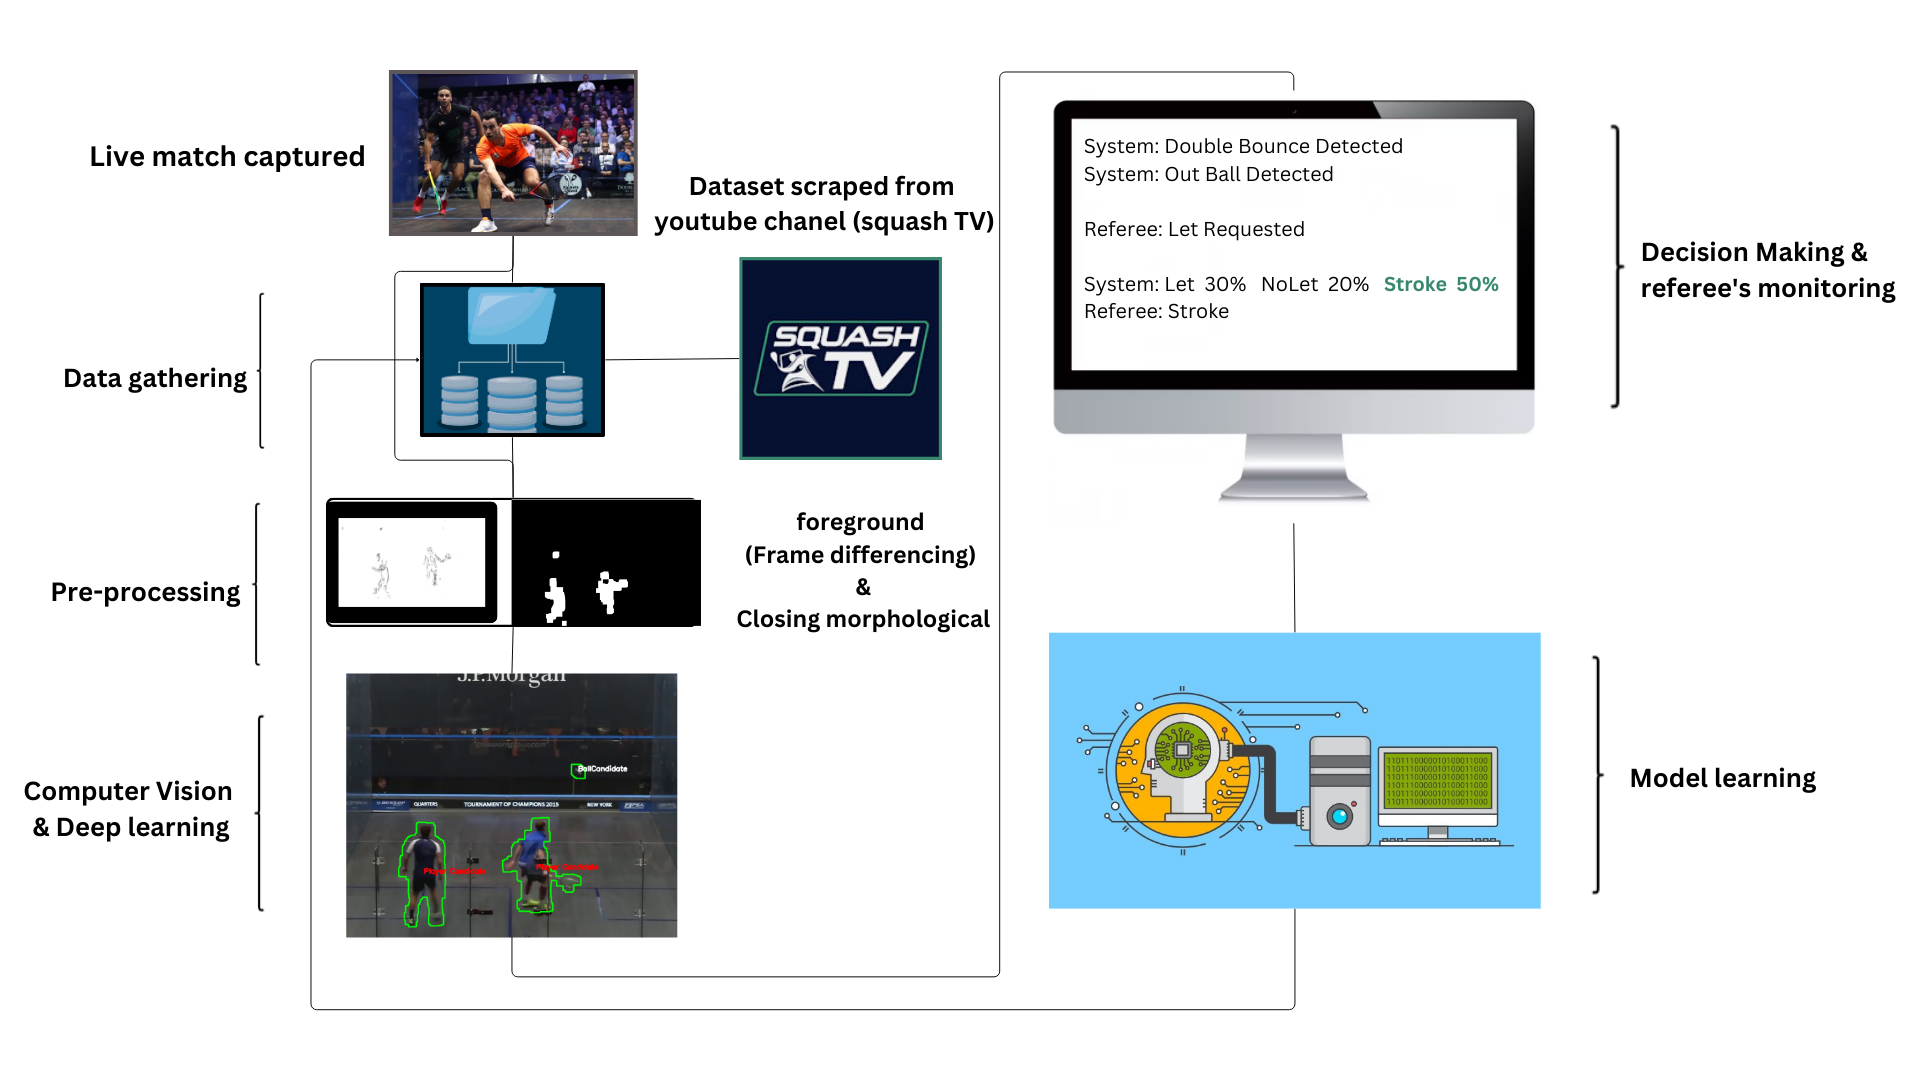
\includegraphics[width=0.80\linewidth]{figures/system overview.png}
    \caption{Over View}
    \label{fig:OverView}
\end{figure}

Figure 2 shows the flowchart of the proposed project. It contains the following steps:
\begin{itemize}
    \item \textbf{input :} A video will be required from a live ongoing match from multiple camera angels. Each camera acts as a single referee, All the cameras will be synchronized and aggregated in a voting system.
    \item \textbf{Data Gathering :} The model is trained on rally videos scraped from youtube channel, the new live match captured by multiple cameras will be used after the match as new data and the data came from the model itself from previous decisions.
    \item \textbf{Pre-Processing :} The main aim at this stage is to extract the foreground of the image frame by subtracting the background from the image.The process involves converting RGB image frames to gray-scale, filtering to reduce noise, combining frames using frame difference and Boolean operations, thresholding to form a binary image, and performing morphological operations like dilation and erosion to enhance objects and minimize discontinuity.
    \item \textbf{Computer Vision \& Deep Learning :} For detection \& tracking the effective ways are Contouring, size, region and velocity constraint.In addition, YOLO and pytorch Achieved a superb outcome. CNN, SVM, LSTM, Transfer learning, GAN and transformers are commenly uesd models.The two methods Kalman Filter \& Holt’s double-exponential smoothing were examined but the accuracy of them cannot be accurately compared due to the lack of ground-truth.(exponential smoothing method results is more smoother and accurate)\cite{squashLowCost}.
    \item \textbf{Decision making \& referee's monitoring :} The system developed decision-making algorithm that fuses data from all cameras making decisions like ball out line and double bounce, but in critical decisions like fouls, the system shows the referee the percentage of the results, and he chooses the right one based on his POV plus the data the system offers. In some cases, if the player feels unfairly judged, the system retests the clash to confirm its decision.
    \item \textbf{model learning :} The model will always keep learning because every match videos is reused as new data. And if the system highest predicted decision didn't match the referee's decision, this case will go to an expert to be checked and the feedback will be returned to the model.

\end{itemize}

% \subsubsection{Data gathering}
% Data gathering is one of the most complicated stages if you do not have a dataset and do not how and where to gather needed data from. In our case their is a couple of data gathering approaches that we can use "Until now".
% Live match captures which means that we can apply a certain amount of cameras in court during live matches to gather our data from different point of views . While the other way by scrapping data from the squash main channel on YouTube "Squash TV".

% \subsubsection{Pre-processing}
% As any usual dataset their is always errors, outliers, and in sufficient data through the dataset. And each type of dataset has its own way to treat this errors. For example: a full numeric dataset that depends on gathering personal info to do some sort of statistics for a scientific purpose first they have check that their is no typing error or empty cells at points that should not happen. Calculating the outliers at salaries rows for example is different to clean text data before modeling it . While, in case of videos and pictures their is different approaches to clean data or to pre-process data. As an example we cant run a model on video as a whole so we need to cut it into specific number of frames per second using some tools like YOLO V8 and many other tools . Then after that we need to prepare this frames to be at ready state for processing .  Salt and pepper noise is one of the most common problems that programmers face while dealing with video-image related systems and one way that it can be solved by using median filter and adaptive total variation model. Plus, an example for preparing data is to sharpen or smooth in image to help in image segmentation.

% \subsubsection {Computer Vision and Deep learning}
\subsection{stakeholder}
\subsubsection{internal}
\begin{enumerate}
\item Ahmed said (Team Leader)
\item Hussein Amr
\item Seif Nasser
\item Youssef Mohamed

%We need to write responsibilities as wellllll!!!!
\end{enumerate}

\subsubsection{external}

\begin{itemize}
 \item  World Squash Federation
 \newline
    FDA is a key stakeholder as it often set rules and standards for refereeing. It may also be involved in approving or regulating the use of such systems in official matches.
 \item Squash Players
  \newline
    Players are directly impacted by the refereeing system.They rely on it to ensure fair and accurate officiating during matches.
 \item Referees
  \newline
    Referees are primary users of the system and are responsible for operating it. Their experience and satisfaction with the system are critical.
 \item Spectators and Fans
  \newline
    They may have an interest in the system if it enhances the viewing experience, such as providing instant replays and statistics.
 \item Investors or Funding Organizations
  \newline
    Investors provide the necessary financial support for the development and implementation of the refereeing system.
\end{itemize}
\section{Similar System}
\subsection{acadimic}

    \begin{itemize}
        \item This paper \cite{squashLowCost} is discussing detecting and tracking fast moving object in squash using low-cost. They have made an important contribution. Using a new dataset they created from Tv brodcast and e broken into rallies of shots manually .Videos have a resolution of 720p and operate at a frame rate of 25 frames per second. The main objective of the preprocessing was to extract the foreground, with adding some filters and threshold to improve the image quality and morphological operations like erosion \& dilated. The results of ball detection using  Contouring, size, region and velocity constraint, evaluated by F1-score with avg. 84.21.performance could be improved with higher fps cameras. For tracking the two methods Kalman Filter \& Holt’s double-exponential smoothing were examined but the accuracy of them cannot be accurately compared due to the lack of ground-truth.(exponential smoothing method results is more smoother and accurate). The challenge they faced that the computational time is 180 milliseconds which exceeds the real-time (40 milliseconds). With required optimization and higher cameras fps the computational time will reduce by 70\%.
     
        \item \textbf{Oussama Tahan, Mohamad Rady, Nabil Sleiman, Milad Ghantous and Zaher Merhi }\cite{8379085}wrote a research paper that focus on analyzing the movement of squash players in court "Footwork" so they can help players to review their mistakes after training, tournaments, etc. They focus on the most important points to consider problems to solve and methodologies that they should use. First, They agreed to use a mid-ranged camera "GoPro HERO3+ Silver Edition" to capture high definition video footage of the game. Plus, the camera has a built in WiFi module so that make it much easier to transfer videos to device easily. However, one of the first challenges that they faced that they had to figure out the best fps to quality ratio to be able to capture a good amount of frames without losing quality. After sending the video from the camera into the device they use FFMPEG tool to extract frames that used for multimedia manipulation to adjust frames and resizing the videos. Then, they had a couple of options on where was the best place to locate the camera. Placing and fixing the camera on top of the glass back wall, adjusting its roll in a way to cover and perceive the players in most of the squash court was the best option. Moreover, they had to use an algorithm so that they can detect players in court so using  Histogram of Oriented Gradients(\textbf{HOG}) to divide frames into small cells and get the gradient direction and then merging cells into regions called blocks to get the block histogram. The set of these block histograms which represents the descriptor. Then after passing these block histograms into Support Vector Machine classifier (\textbf{SVM}) to detect players. On the other hand, this paper had a couple of withdraws like they are not a real time system they depend on sending the video to the processor after the match ends so the players can see their weaknesses after the match in a simple UI. And for last the fact that they are using the player's t-shirt color to recognize the players is a problem because it is very possible for both players to wear the same color. 
        \begin{figure}[H]
            \centering
            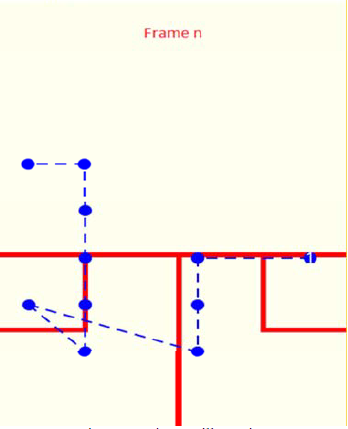
\includegraphics{figures/figure 1.PNG}
            \caption{Trajectory illustration}
            \label{fig:enter-label}
        \end{figure}

        \item \textbf{Nady, Xiang Li}\cite{9163908} wrote a research paper that initiate a big move in the world of Artificial Intelligence Specially at classical decision making algorithms that just agree on using an specific available action and Markov model which decides their actions after sorting it sequentially. Instead of that they decided to model a module that can give the most optimal decisions with assumption of insufficient knowledge and resource while using the old algorithms too. Additionally The proposed model is a heuristic-primed decision-making model that mainly implements the mechanism of choosing beliefs, wishes, and action plans. But, the paper compares its own methods with the computer implementation and in term in fuctions of the  Non-Axiomatic Reasoning System \textbf{NARS} The proposed model is simulated in an urban firefighting case, and the uncertain information in every aspect of the model is represented by a unified method using NAL Which is separated to 9 different layers but on their paper they used only the first 6 layers and each layer introduce either different type of variables or rules. Finally, each layer belongs to specific term Atomic term (NAL-1) , Compound term (NAL-1, NAL-2, NAL-3, NAL-4), and High-order term (NAL-5, NAL-6). And a big drawback about this paper that they did not mention or use any data-sets ,instead they used a case-study for a firefighting scenario so you can imagine how does the process of the decision making works.
        
        \item \textbf{Zhihao Chen, Redouane Khemmar, Benoit Decoux, Amphani Atahouet, and Jean-Yves Ertaud} \cite{8806222} wrote a research paper that helps people with disabilities specially on wheelchair improve the efficiency of chair by making a system for low-consumption platforms and with a low-cost materials so it could be applicable to apply on wheel chairs. Going through the paper he made a lot of comparisons. At first he made a comparison between one-stage methods , which provide estimation of position and estimation of classes in one step for example (\textbf{You Only Look Once "YOLO", and Single Shot Detector "SSD"}),
        while, two-stage methods first detect regions of the images where object could be present, and then apply these regions to a classifier for example (\textbf{Region-proposal Convolutional Neural Network "RCNN"}). As a result, after testing both methods they found out the one-stage methods was faster than two-stage method and with similar accuracy. After that they started to compare between three different approaches YOLO , SSD , and Faster-RCNN and with the same order mentioned the accuracy was increasing while, speed was decreasing. Since it is a real time system speed was an important factor so they decided that SSD was better approach since their was neither big of a difference between SSD and Faster RCNN accruracy nor a huge gap between SSD and YOLO's speed that was before a better version of YOLO V3 approached. The model of the SSD that they evaluated was trained with the PascalVOC learning base. While the YOLO V3 model they evaluated was trained with the Coco learning base. And YOLO V3 results was better in case of speed and \textbf{ Mean Average Precision "MAP"}. Then they started to think of ways to calculate distance between camera and object so they used the Monodepth algorithm which is trained on stereo images dataset but its inference uses monocular images that gives a disparity map as its output that they have trained with different backbones including (\textbf{VGG and ResNet}) through two different datasets (\textbf{Cityscape and Kitty}). Then they merge the output of the disparity map and the object detection to give them higher efficiency. 

        \item
        In the article entitled \textbf{Unsupervised Temporal Feature Aggregation for Event Detection in Unstructured Sports Videos} \cite{8959041}, the authors presented and focused on a new technique for heuristic score boosting using feature aggregation-based outlier rejection for player improvement without any user interface. The method primarily focused on the issue of rally detection in table tennis videos captured from arbitrary camera angles with real-time performance (10--25 FPS) to allow human analysts to summarize the game as soon as it ends. The authors then highlight two major problems related to the application. Firstly, there is no access to player bounding box annotations during training, requiring unsupervised player capture retrieval from each image frame without any user intervention. The second problem they faced is that the dataset has high variation in camera pose but limited variations in appearance features such as color, making it prone to overfitting. The authors mentioned that the proposed method uses player-level image features to classify whether a window of video frames belongs to a rally event or not. They also implemented a data augmentation method using an image translation model, retaining the base content of the samples while increasing variability in appearance features to improve model generalization to unseen test cases. According to some experimental evaluations, the authors indicated that the proposed temporal feature aggregation method can enhance the precision of player retrieval. Similarly, the rally detector model trained using player-level features can improve the F1 Score from 0.79 to 0.89 when compared to the baseline global frame-level feature-based detectors. In conclusion, the paper presented a real-time automatic rally scene detection method from unstructured table tennis videos shot at arbitrary camera angles in an efficient way, and the researchers successfully proved their point of view.
        
        \item In the article entitled \textbf{Evaluation of Open-Source and Pre-Trained Deep Convolutional Neural Networks Suitable for Player Detection and Motion Analysis in Squash} \cite{s21134550} the authors Christopher Brumann, Markus Kukuk, and Claus Reinsberger mainly focused on the use of deep convolutional neural networks for player detection and motion analysis in the sport of squash and they mainly focused on how many CNNs available for out-of-the-box inference on squash data for motion analysis by conducting an investigation that was systematic over 250 CNNs. They took the most suitable three that met their criteria of being pre-trained, open source, and they were ready to use. The authors also focused on the extent and the accuracy to these CNN models and their allowance motion analysis in squash, by crating a labelled dataset by manually annotating videos of squash matches. They also developed by making a labeling tool to annotate detet and annotate the players’ feet positions. Also they tested and evaluated the capabilities and performance of the selected three CNNs by sing the labelled datasets. They found at the end that the CNNs were accurate and robust against acclusion, which is happening regularly in the rally situation. The researchers also focused on the data that was obtained from the CNNs to be easily used to provide enough and useful insights to the coaches and also to the athletes by developing a heaatmap visualization technique which used to display the spatial distribution of player locations on the court. this was so helpful as the visualization was used to compare the CNN detections with the ground truth tables and gave good results, also the type of the court is a really important point to be considered when analyzing squash matches. The authors found at the end that CNN models can be effectively used for player detection and motion analysis for squash in general and helpful to the players. Also the selected CNNs were so accurate sufficiently on a squash dataset specifically, and the heatmap visuaalization technique was so helpful and useful to be used to provide enough and valuable information to the coaches and the athletes.

        \item In the article entitled \textbf {Tracking Fast Moving Objects by Segmentation Network} \cite{9413129}. The authors are presenting a new approach to tracking fast-moving objects in video sequences using modern deep-learning methods. the method is mainly focused on tracking the object by segmentation approach, where the object is segmented from the background in each frame of the video sequence, and the segmentation of the result is used to track the object's trajectory over time. The authors discussed then the challenges they faced in tracking fast-moving objects as motion blur, occlusions, and changes in appearance due to lighting conditions. They discussed the solution they found which dials into small bright foregrounds and demonstrates the possibility of fast model fine-tuning for different foreground types. The authors then found and proposed a method for evaluating the FMO dataset, which shows competitive results compared to other state-of-the-art methods for precision and execution time. they also investigated cases where the algorithm performs out or under current methods. They discussed a detailed description of the method, and also the FMO sequence generator used for training,  the segmentation network architecture, and the fine-tuning process for different foreground types. The authors also mentioned the potential applications of the segmentation results such as trajectory prediction and de-blurring algorithms. The paper shows a promising approach to track fast-moving objects by using modern deep-learning methods and also demonstrates the effectiveness of the FMO dataset. The method they mentioned has a potential to be adapted for different foreground types and was applied to more than a scenario. 

       \item 
       This paper \cite{9289223} discusses tracking and analysing the movements of players by deep learning. It shows multiple image processing algorithms for player tracking.They perform an experiment using a network that uses the item's centre point rather than its bounding box for object tracking and simultaneously carries out object detection and object identification.Each object was educated by taking 760 randomly selected continuous frames from an American football (KIM
       \item CHI-BALL) film in order to add more learning.. 
        The experiment was conducted in the following environment
        \begin{itemize}
             \item OS: Ubuntu 18.04
             \item Development languages and tools:\\
             Python 3.7, Pytorch 1.4, CUDA 10.1, CuDNN 7.6.5
             \item GPU: RTX 2080 x 4 
        \end{itemize}
        The model success rate of detection and tracking of players is 
        significantly increased in Fig 1. after additional learning about the 
        players in the field.The model is also applied on soccer video and it shows a significant improve.Through this, it was found that the number of pixels occupied 
        by the object in the image used for learning or the resolution 
        of the image affects object tracking.
        \begin{figure}[H]
            \centering
            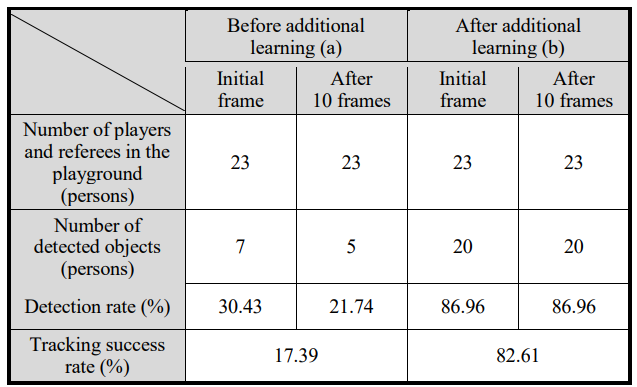
\includegraphics{figures/Screenshot 2023-11-11 193421.png}
            \caption{KIMCHI-BALL}
            \label{fig:KIMCHI-BALL Output}
        \end{figure}

        \item 
        In the paper entitled \textbf {Event-Based High-Speed Ball Detection in Sports Video} \cite{10.1145/3606038.3616164} written by \textbf {Nakabayashi, Takuya and Kondo, Akimasa and Higa, Kyota and Girbau, Andreu and Satoh, Shin'ichi and Saito, Hideo} it talks about detecting fast moving balls in sports, they are working on volleyball sport for applying their techniques, it introduced another approach for detecting fast moving balls by using another type of cameras that is called event camera that works in a different way than a normal camera, They contributed in the data-set and proposed two methods; using an event camera for generating a data-set and using events generated from the common camera, the methods they proposed showed an outstanding in the results compared to others, the paper has a new technique which is great but it faces a challenge in the data-set as it is limited and they are using YOLOV3(You Only Look Once) which is fine but YOLOV8 has more accuracy.  
 
        \item 
        In the paper entitled \textbf {VARS: Video Assistant Referee System for Automated Soccer Decision Making from Multiple Views} \cite{10208684} written by \textbf {Held, Jan and Cioppa, Anthony and Giancola, Silvio and Hamdi, Abdullah and Ghanem, Bernard and Van Droogenbroeck, Marc} the main goal is to automate the referee decisions based on multi-view video and be accurate and eliminate human error in order to ensure fairness, the authors collaborated to solve the problem of refereeing and contributed with their own multi-view data-set named SoccerNet-MVFouls, making the VAR system using multi-view for classifying and proposed in this paper how different camera can affect the performance of the system. The system showed great results with the different classifiers and transformers like ResNet, CNN R(2+1D), and MVit, The paper includes a challenge and has been solved in a good approach which is multi-view refereeing and it eliminated the human error by showing the fouls in different point of views it faced some challenges but managed to overcome it.

        \item In the article entitled \textbf {Wiimote Squash: Comparing DTW and WFM  Techniques for 3D Gesture Recognition}\cite{wiimote}, the authors mainly focused on the effectiveness of DTW and WFM techniques in detecting 3D gestures in a Squash game application using the Wiimote. The authors started the paper by discussing the importance of gesture recognition in computing environments and how it can be usefully used to augment our feelings, emotions, social integration, and communication. The writers also talked about the importance of the differences and challenges between gestures performed on physical devices such as the Wiimote and Playstation controller, which shows that these devices perform in the air and require different handling for their detection recognition. The authors also explained the Squash game application used in this study and how it works with the Wiimote. They showed that the 5 techniques implemented for different squash shots performed a controlled experiment to compare the recognition accuracy of DTW and WFM. The results showed that there was no significant difference in the recognition of DTW and WFM for Wiimote gestures. These results showed the effectiveness of existing gesture recognition techniques and highlighted the potential for use in 3D gesture recognition applications. Moreover, the paper discussed the potential for extending the vocabulary of gestures and enhancing the application of the Kinect game console as the writers suggested that future research could explore the use of semantic technologies, ontology-enabled context management, and augmented reality to further enhance and improve the application and its usability. The paper then continues to contain some related work, the design of the Squash game court, the working of Wiimote, Wiimote pointing, the Squash game developed, the experiment and results, the comparison of existing techniques with the current work, and future work. To conclude, the paper enhanced valuable insights into the effectiveness of DTW and WFM techniques for 3D gesture recognition in a specific application and highlights potential areas for future research.

        \item In the article entitled \textbf{Evolution Based Single Camera Resectioning Based on Distance Maps of a Known Geometry for Squash Sports} \cite{9784855} by C. Brumann and M. Kukuk. The authors discussed and mentioned a genetic algorithm implementation that can be used for camera calibration in both prospective and retrospective manners. They mentioned that the algorithm would be very useful to help coaches and people who make analyses to the game gain insight into training quality and allow for better training control. Then the authors mentioned the area with the highest importance on the court floor, called the T area. It appears that controlling this area relates to a player's dominance during a rally and ultimately with the likeliness of winning that rally. Moreover, They mentioned that the awareness of the opponent's motion is essential to retaining control of a rally. The writers mentioned that the game requires quick reactions to the opponent's actions, and there remains only a short time for making tactical decisions. Also, as a skill to improve, you have to internalize certain patterns in training and retrieve the pattern in competition. They also discussed a recent study that showed six situation awareness clusters, including players' positions on the court, and found differences in expert athletes' behavior. They mentioned that the topic is very important for elite squash athletes as individual locations on the playing field may also reveal individual strengths and weaknesses during match play and allow investigation of athletes' performances during training. The paper also contains references to other studies that have been conducted on squash sports. These studies include a review of the performance requirements of squash, specifications for squash courts, and dynamic patterns of movement of squash players of different standards in winning and losing rallies. In conclusion, this Paper proofs valuable and meaningful information on the evolution based on Single Camera resectioning for Squash sport. The genetic algorithm implementation can be used for camera calibration in both prospective and retrospective manners, allowing coaches and analysts to gain the value they need in training quality and better training control. Moreover, the importance of the T area and awareness of the opponent's motion were also discussed, besides the significance of internalizing certain patterns during training and applying them in competition. 

        \item 
        This paper introduces the Need for Speed benchmark\cite{need_for_speed}, which is a new dataset and benchmark for visual object tracking.(from their knowledge) it is the fisrt benchmark for higher frame rate general object tracking. This dataset consists of 100 videos (380K frames) captured with now commonly available higher frame rate (240 FPS) cameras like iphone 6 and above from real world scenarios and tracking targets include vehicle, person, face, animal, boat and generic objects (e.g.\textbf{ sport ball}, cup, bag, etc.).The tracking methods is generally divided into two categories, including correlation filter (CF) trackers[BACF,CSRDCF,C-COT,CF2,CFNet,DAT,ECO,KCF,LCT,MCCT,MEEM,MDNet,SRDCF] and deep trackers[MDNet,SiamFC,SiamRPN]and used on diffrent tracking Datasets. The used Evaluating Algorithms was :
        \begin{itemize}
            \item Correlation Filter (CF) trackers with hand-crafted features:         BACF, SRDCF, Staple, DSST, KCF, LCT, SAMF, and CFLB.
            \item CF trackers with deep features: HCF and HDT.
            \item Deep trackers: MDNet, SiameseFc, FCNT, and GOTURN.
        \end{itemize}
        The effect of capture frame rate on tracking performance was measured by two different tracking scenarios.In the first scenario, each tracker is tested on the Need for Speed dataset at both 30 frames per second (FPS) and 240 FPS. The second scenario involves testing the trackers on a dataset with synthesized motion blur and a dataset with real motion blur, both captured at 30 FPS.
        \begin{figure}[H]
        \centering
        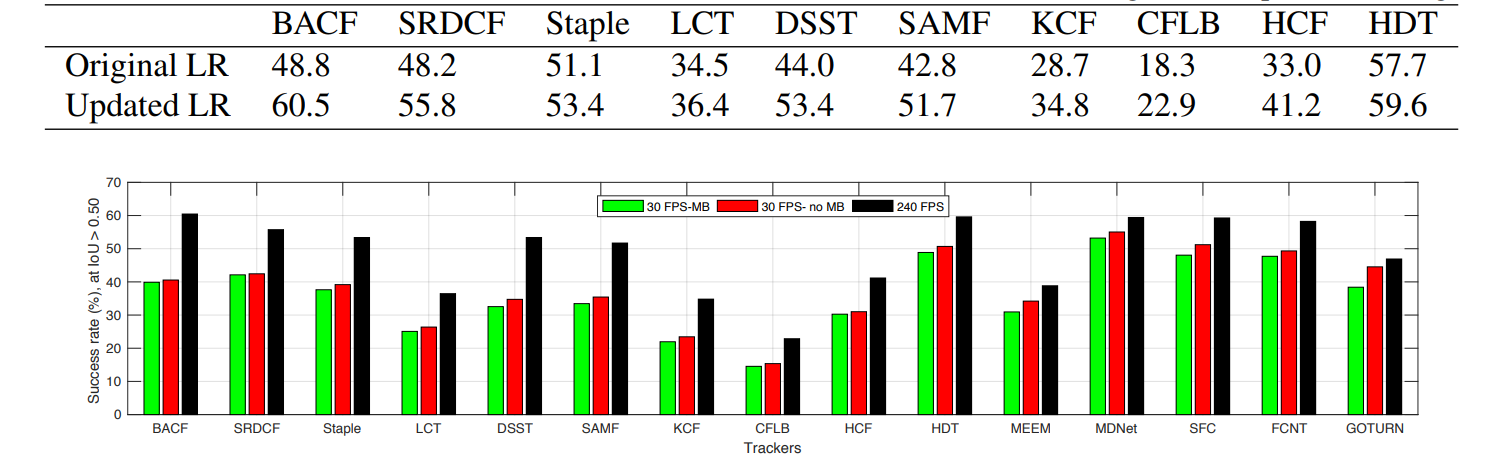
\includegraphics[width=1\linewidth]{figures/Need for Speed results.png}
        \caption{Comparing higher frame rate tracking (240 FPS) versus lower frame rate tracking (30 FPS) for each tracker. }
        \label{fig:Comparing higher frame rate tracking (240 FPS) versus lower frame rate tracking (30 FPS) for each tracker. }
        \end{figure}
        Surprisingly, the results show that at higher frame rates, simple CF trackers with hand-crafted features outperform complex deep trackers in terms of both accuracy and computational efficiency.This dataset fills a need, the need for speed.

        \item in the master thesis entitled \textbf{"Deep learning applied to detection, pose estimation, tracking, and birds-eye view in sport videos"}\cite{upm75832} it discusses different solutions for different data science processes problems, so the thesis contributed by providing a comprehensive analysis of different techniques used to develop detection models pose estimation, tracking, and bird's eye view in sports, it used YOLOv7 and MediaPipe for detection and put in consideration Faster R-CNN, SSD, and Mask R-CNN, For tracking it used different algorithms like SORT, DeepSORT, and ByteTrack also put in consideration other algorithms like MHT(MUltiple Hypothesis Tracking), Kernalized Correlation Filters(KCF) and Online Multi-Object Tracking (MOT), And for pose estimation it used YOLOv7-pose and suggested OpenPose, MediaPipe and HRNet, And for birds-eye view it used pre-trained model that uses two-GAN networks and suggested other methods like Direct Linear Transform(DLT) and Random sample consensus(RAN-SAC), The thesis used three different data-sets COCO data set, Basketball game and football game data-set, The results showed a successful achievement of it's objectives, The paper is full with different techniques but it needs to optimize the models for real-time processing and the difficulty of obtaining high-quality training data.
        \begin{figure}[H]
        \centering
        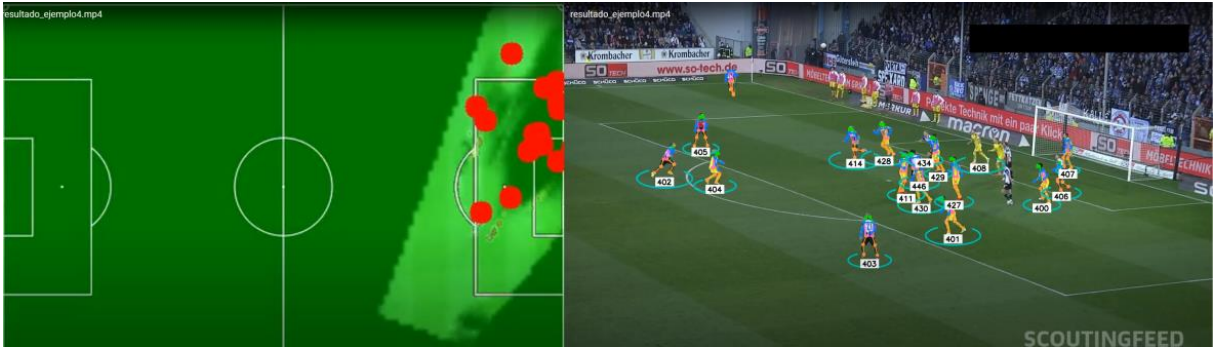
\includegraphics[width=1\linewidth]{figures/fig1.png}
        \caption{example of the results}
        \label{fig:example of the results. }
        \end{figure}

        \item in the article entitled \textbf{Deep learning in multi-object detection and tracking: state of the art}\cite{Pal2021-re} written by \textbf{Sankar K. Pal1 · Anima Pramanik2 · J. Maiti2 · Pabitra Mitra3} it provide a comprehensive study on deep learning-based object detection and tracking, including the analysis of suitable combinations of detectors and trackers for different types of data. it used different algorithms like YOLO(different versions, v2, v3), CNN ,Faster RCNN, Mask RCNN, SSD (Single-shot detector) , DSSD (De-convolutional Single Shot Detector), FPN(feature pyramid network), R-FCN, DCN(Deformable convolutional networks), AMIR, Deep SORT, MHT-DAM, CDA-DDAL, RNN-LSTM, QuadMOT, STAM-MOT, and Siamese CNN. They used different data-sets like PASCAL VOC, MS COCO, ImageNet and MOT,but in the end, yolo was the fastest model, They faced some challenges like the need for large amounts of annotated data, the difficulty of handling occlusions and cluttered scenes, the need for real-time processing, and the trade-off between accuracy and speed. The paper can be reliable or taken as a reference for different models approaches and techniques as it explains each model and it's alternatives in detail.
                \begin{figure}[H]
        \centering
        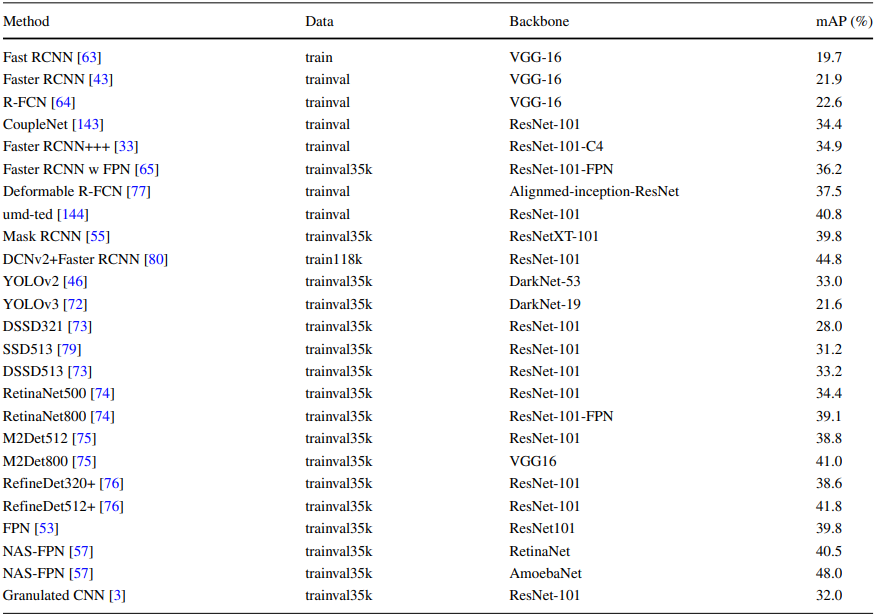
\includegraphics[width=1\linewidth]{figures/detection ms coco.PNG}
        \caption{Detection results of various general object detectors over MS COCO test-dev dataset}
        \label{fig:Detection results of various general object detectors over MS COCO test-dev dataset. }
        \end{figure}

                \begin{figure}[H]
        \centering
        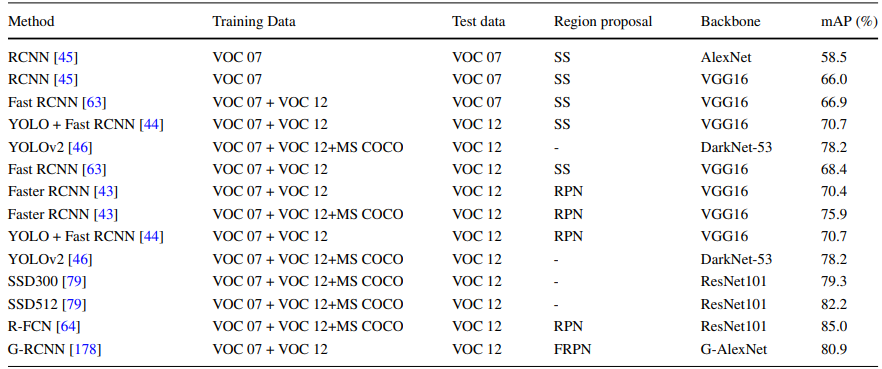
\includegraphics[width=1\linewidth]{figures/detection pascal voc.PNG}
        \caption{Detection results of various detectors over PASCAL VOC dataset}
        \label{fig:eDetection results of various detectors over PASCAL VOC dataset }
        \end{figure}

        \item in the article entitled \textbf{"Understanding of Object Detection Based on CNN Family and YOLO"} \cite{Du_2018} written by \textbf{"Juan Du"} provides a comparison between two popular algorithms used in the detection and tracking of objects and these algorithms are YOLO and CNN Family, The problem the paper is trying to solve is related to image processing classification and localization, the researcher used PASCAL VOC and MS COCO data-sets, The results are shown the figure below, the challenges that appeared are the requirements of high computing capability of the hardware,the paper showed a great comparison between YOLO and CNN family and FAST YOLO was the supreme in this paper.
        \begin{figure}[H]
        \centering
        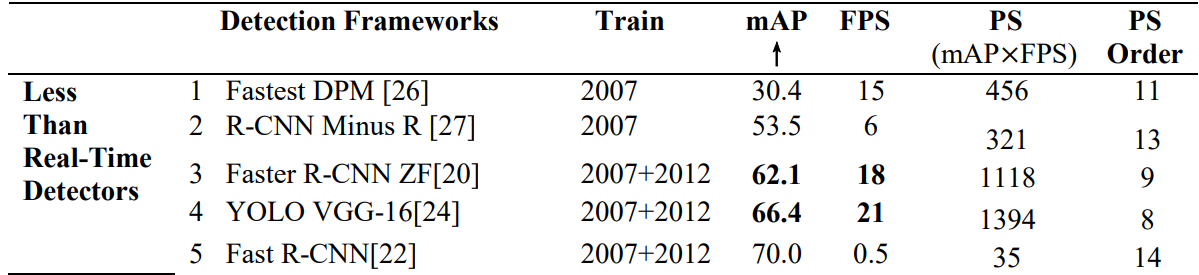
\includegraphics[width=0.75\linewidth]{figures/det1.PNG}
        \caption{The Performance Compare of the Detection Systems.}
        \label{fig:The Performance Compare of the Detection Systems. }
        \end{figure}
        \begin{figure}[H]
        \centering
        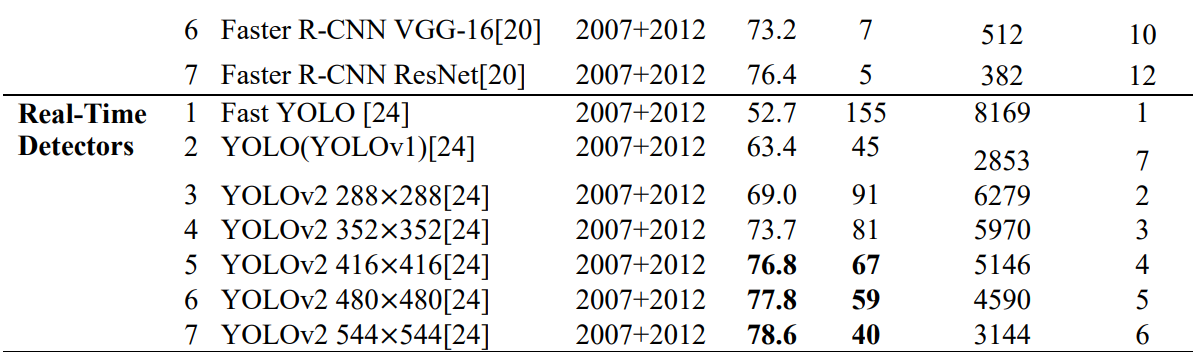
\includegraphics[width=0.75\linewidth]{figures/det2.PNG}
        \caption{The Performance Compare of the Detection Systems.}
        \label{fig The Performance Compare of the Detection Systems. }
        \end{figure}

        \item in the article entitled \textbf{"Online detection and classification of in-corrected played strokes in table tennis using IR depth camera"} written by \textbf{"Habiba Hegazy and Mohamed Abdelsalam and Moustafa Hussien and Seif Elmosalamy and Yomna M.I Hassan and Ayman M. Nabil and Ayman Atia"} it talks about detection of table tennis strokes using IR depth camera, They focus on player's performance measures, they analyze the data collected from the IR depth camera by using fastDTW algorithm, they made their own data-set, The results showed the highest accuracy with FastDTW and KNN,SVM and Naive Bayes showed less accuracy, The paper showed good algorithms and techniques for detection and classification of game strokes but it faces a challenge because of the rare data-set of tennis 
        
        \begin{figure}[H]
        \centering
        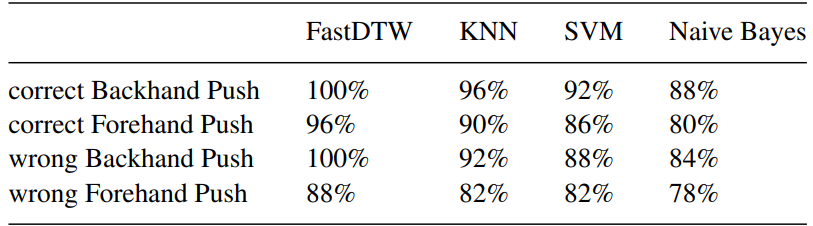
\includegraphics[width=0.75\linewidth]{figures/detres.PNG}
        \caption{Different classification algorithm comparison.}
        \label{fig Different classification algorithm comparison}
        \end{figure}

    \item in the article entitled \textbf{"The MTA Dataset for Multi Target Multi Camera Pedestrian Tracking by Weighted Distance Aggregation"} \cite{9151039} written by \textbf{"Köhl, Philipp and Specker, Andreas and Schumann, Arne and Beyerer, Jürgen"} it talks about multi-target and multi-camera tracking, they faced a challenge with the real world data-set as it requires the guaranty of the privacy, so the authors created their own data-set from a video game with 2,800 person identities,6 video cameras and a video of length over 100 minutes per camera and name the data-set MTA(Multi Camera Trach auto) they also used different algorithms for their project, they used FRCNN for person detection and CNN for person re-identification and other algorithms like hierarchical clustering, correlation clustering, kalman filter, intersection over union(IOU), DeepSORT,YOLO, RetinaNet and Cascade R-CNN, for multi-target camera they proposed weighted distance aggregation approach as it showed a great result and for object identification they used faster R-CNN, this paper showed a comprehensive comparisions for multi camera tracking the main problem was the data-set
        \begin{figure}[H]
        \centering
        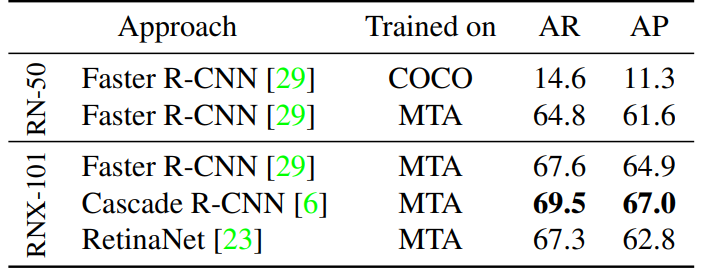
\includegraphics[width=0.75\linewidth]{figures/tdet.PNG}
        \caption{Person detection evaluation results on the MTA dataset.}
        \label{fig Person detection evaluation results on the MTA dataset.}
        \end{figure}

    \end{itemize}
    
\subsection{business Application}

\begin{enumerate}
% add ref
    \item Hawk-Eye \cite{Hawk-eye}: Hawk-Eye is a computer vision system that is used to visually track the trajectory of the ball and display a profile of its statistically most likely path as a moving image. It is used in various sports, including volleyball, association football, badminton, hurling, rugby union, and cricket. Shot Spot is the term for the trajectory findings' on-screen depiction.
        \begin{figure}[hbt!]
            \centering
            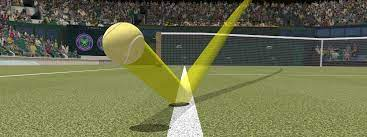
\includegraphics{figures/hawk-eye decision.jpeg}
            \caption{Hawk-eye Shot Spot}
            \label{fig:hawk-eye}
        \end{figure}
        \newpage

    \item The video assistant referee \cite{var}: (VAR) is a match official in association football who assists the referee by reviewing decisions using video footage and providing advice to the referee based on those reviews.
        \begin{figure}[hbt!]
            \centering
            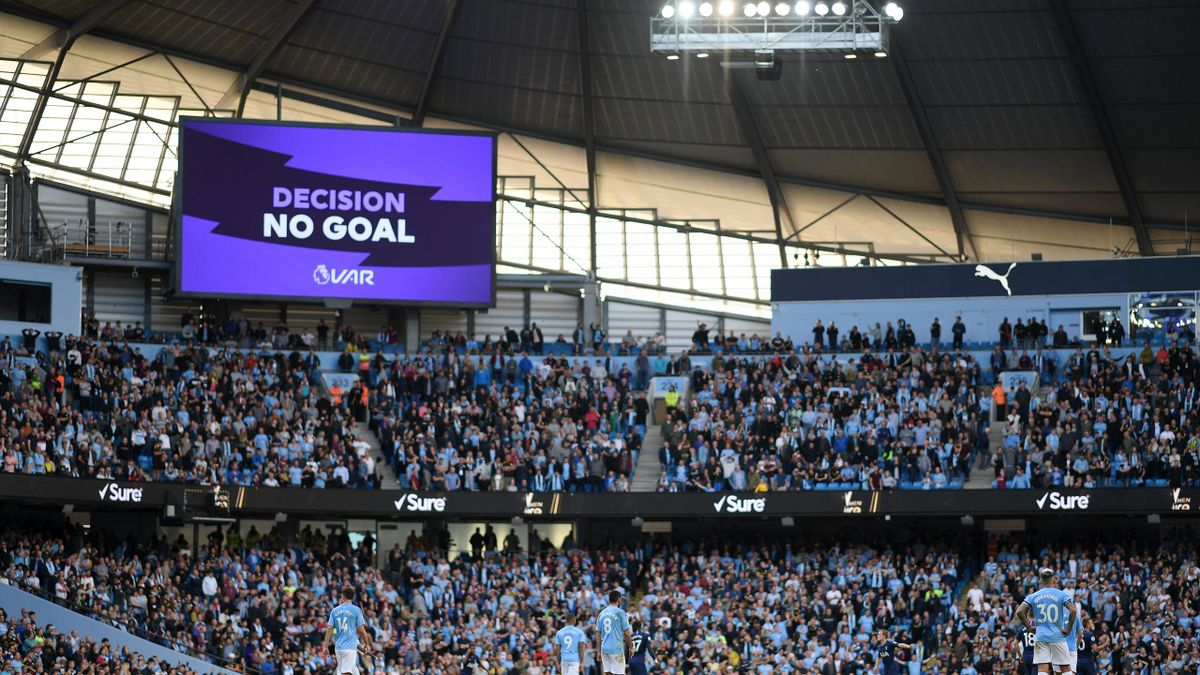
\includegraphics[width=0.6\linewidth]{figures/var-decision.jpg}
            \caption{VAR}
            \label{fig:enter-label}
        \end{figure}
    \item Sevensix \cite{sevensix}: Sevensix is an AI-powered app that analyzes your tennis technique to help you upgrade your game.
        \begin{figure}[hbt!]
            \centering
            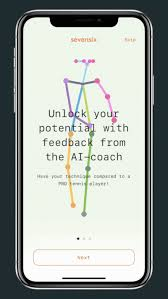
\includegraphics{figures/sevensix app.jpeg}
            \caption{Sevensix app}
            \label{fig:sevensix app}
        \end{figure}



\end{enumerate}

\newpage
\section{What is new in the Proposed Project?}
Our Squash refereeing system introduces a radical departure from conventional methods.By leveraging Computer Vision, data analytics and Machine Learning.Through advanced algorithms, our system tracks the ball's position, player movements and critical match events. We have created a system that allows for accurate and fair officiating during squash matches by making decisions in real-time, both autonomously and semi-autonomously. Our technology is unique among traditional refereeing techniques because of its autonomous capability, which promises to improve officiating accuracy and efficiency while providing players and spectators with a smooth, unbiased experience.With a commitment to innovation and technological advancement, our Squash Refereeing System is poised to redefine the standards of fairness and objectivity in the sport of squash.

 \subsection{Challenges}
We faced few obstacles and we managed to overcome to carry out this project: 
\begin{itemize}
\item One of them is the lack of ready made datasets to use to train our model 

\item The database size used to support this system.

\item Real time processing is not easy. One of the similar systems has reached 180 milliseconds computational time for only preprocessing ,detecting and tracking. which is very high for real time computation (40 milliseconds).

\item The cameras already used does not meet the specs that we need. 

\item Also the high speed of the ball makes it much harder to be detected and tracked,putting in consideration the need to synchronize all of these cameras to a single decision.

\item Finally ,the main challenge that we are facing is that this idea has not been proposed before.
\end{itemize}
 \subsection{Contribution}
 \begin{itemize}
 \item We managed to overcome the datasets problem by collecting YouTube videos for squash matches recorded from the Professional Squash Association (\textbf{PSA}) and gathering some refereeing videos from the World Squash Officiating (\textbf{WSO}) website with their ground truth proving that the referees used to have wrong decisions.

 \item We Considered using a database that supports efficient storage and retrieval of large binary objects (BLOBs) like videos (MongoDB).The Design of the database schema will accommodates metadata about the videos (e.g. title, ground truth). Google Cloud Storage will be used as a dedicated file storage solution for storing the actual video files.

 \item High performance processor with optimizations like (Neon ,VF pv3 \& reducing the video resolution to 480p) and high RAMs will reach our desired time. 

 \item For model training we will work hardly to cope with the available cameras but for testing cameras with 60 frames per second or higher will be much preferred.

 \item All cameras shall be time and frame synchronized \cite{Multiple_Cameras} by NTP and aligning the frames to common timeline. Cameras calibration and common coordinate system with
 implementing efficient communication protocols.Developing a decision-making algorithm that fuses data from all cameras to reach a unified decision.

 \item Thus the limited literature and uncertain methodologies requires resilience, creativity, and effective problem-solving.
 \end{itemize}


\section{Proof of concept}
    \begin{figure}[H]
        \centering
        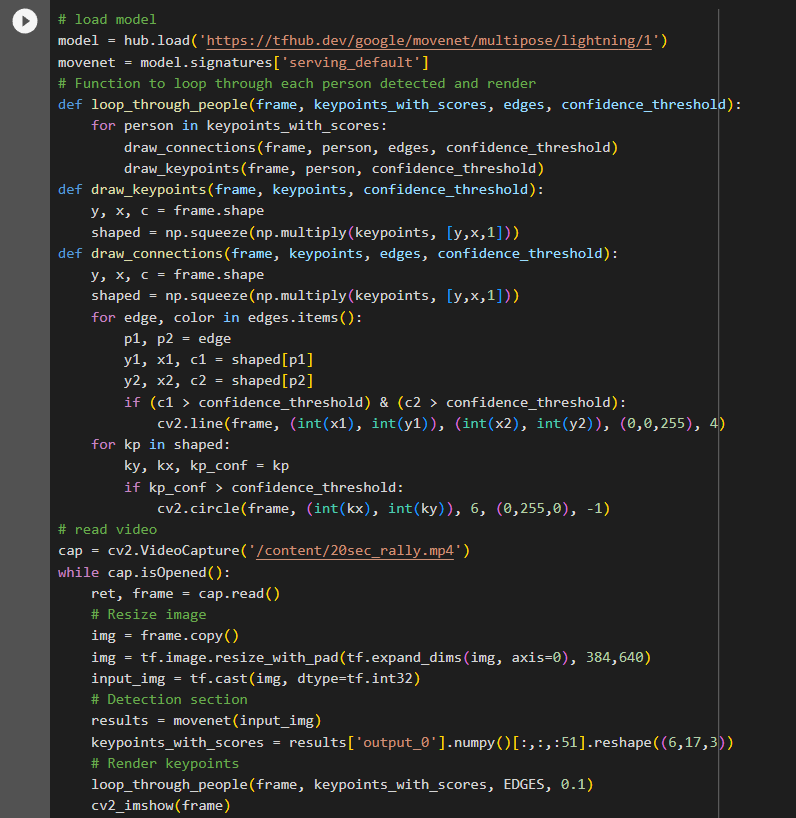
\includegraphics[width=1\linewidth]{figures/humen-pose-code.png}
        \caption{Person Tracking}
        \label{fig:person tracking}
    \end{figure}
    \begin{figure}[H]
        \centering
        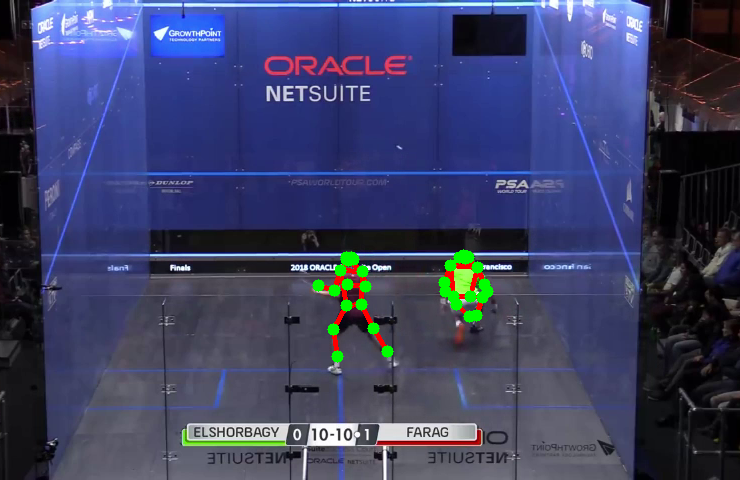
\includegraphics[width=1\linewidth]{figures/humen-pose-output.png}
        \caption{Person Tracking Output}
        \label{fig:peson tracking output}
    \end{figure}

    \begin{figure}[H]
        \centering
        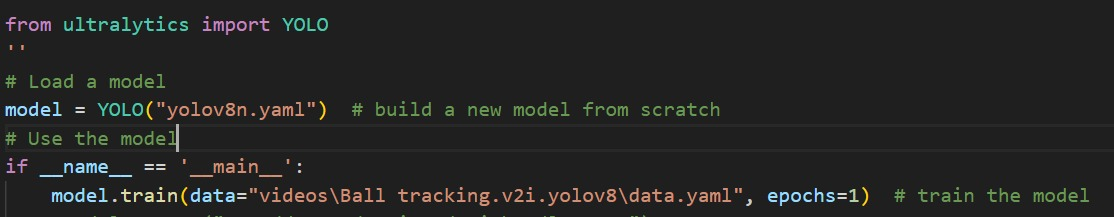
\includegraphics[width=1\linewidth]{figures/ball tracking.jpg}
        \caption{Ball Tracking}
        \label{fig:Ball tracking}
    \end{figure}
    \begin{figure}[H]
        \centering
        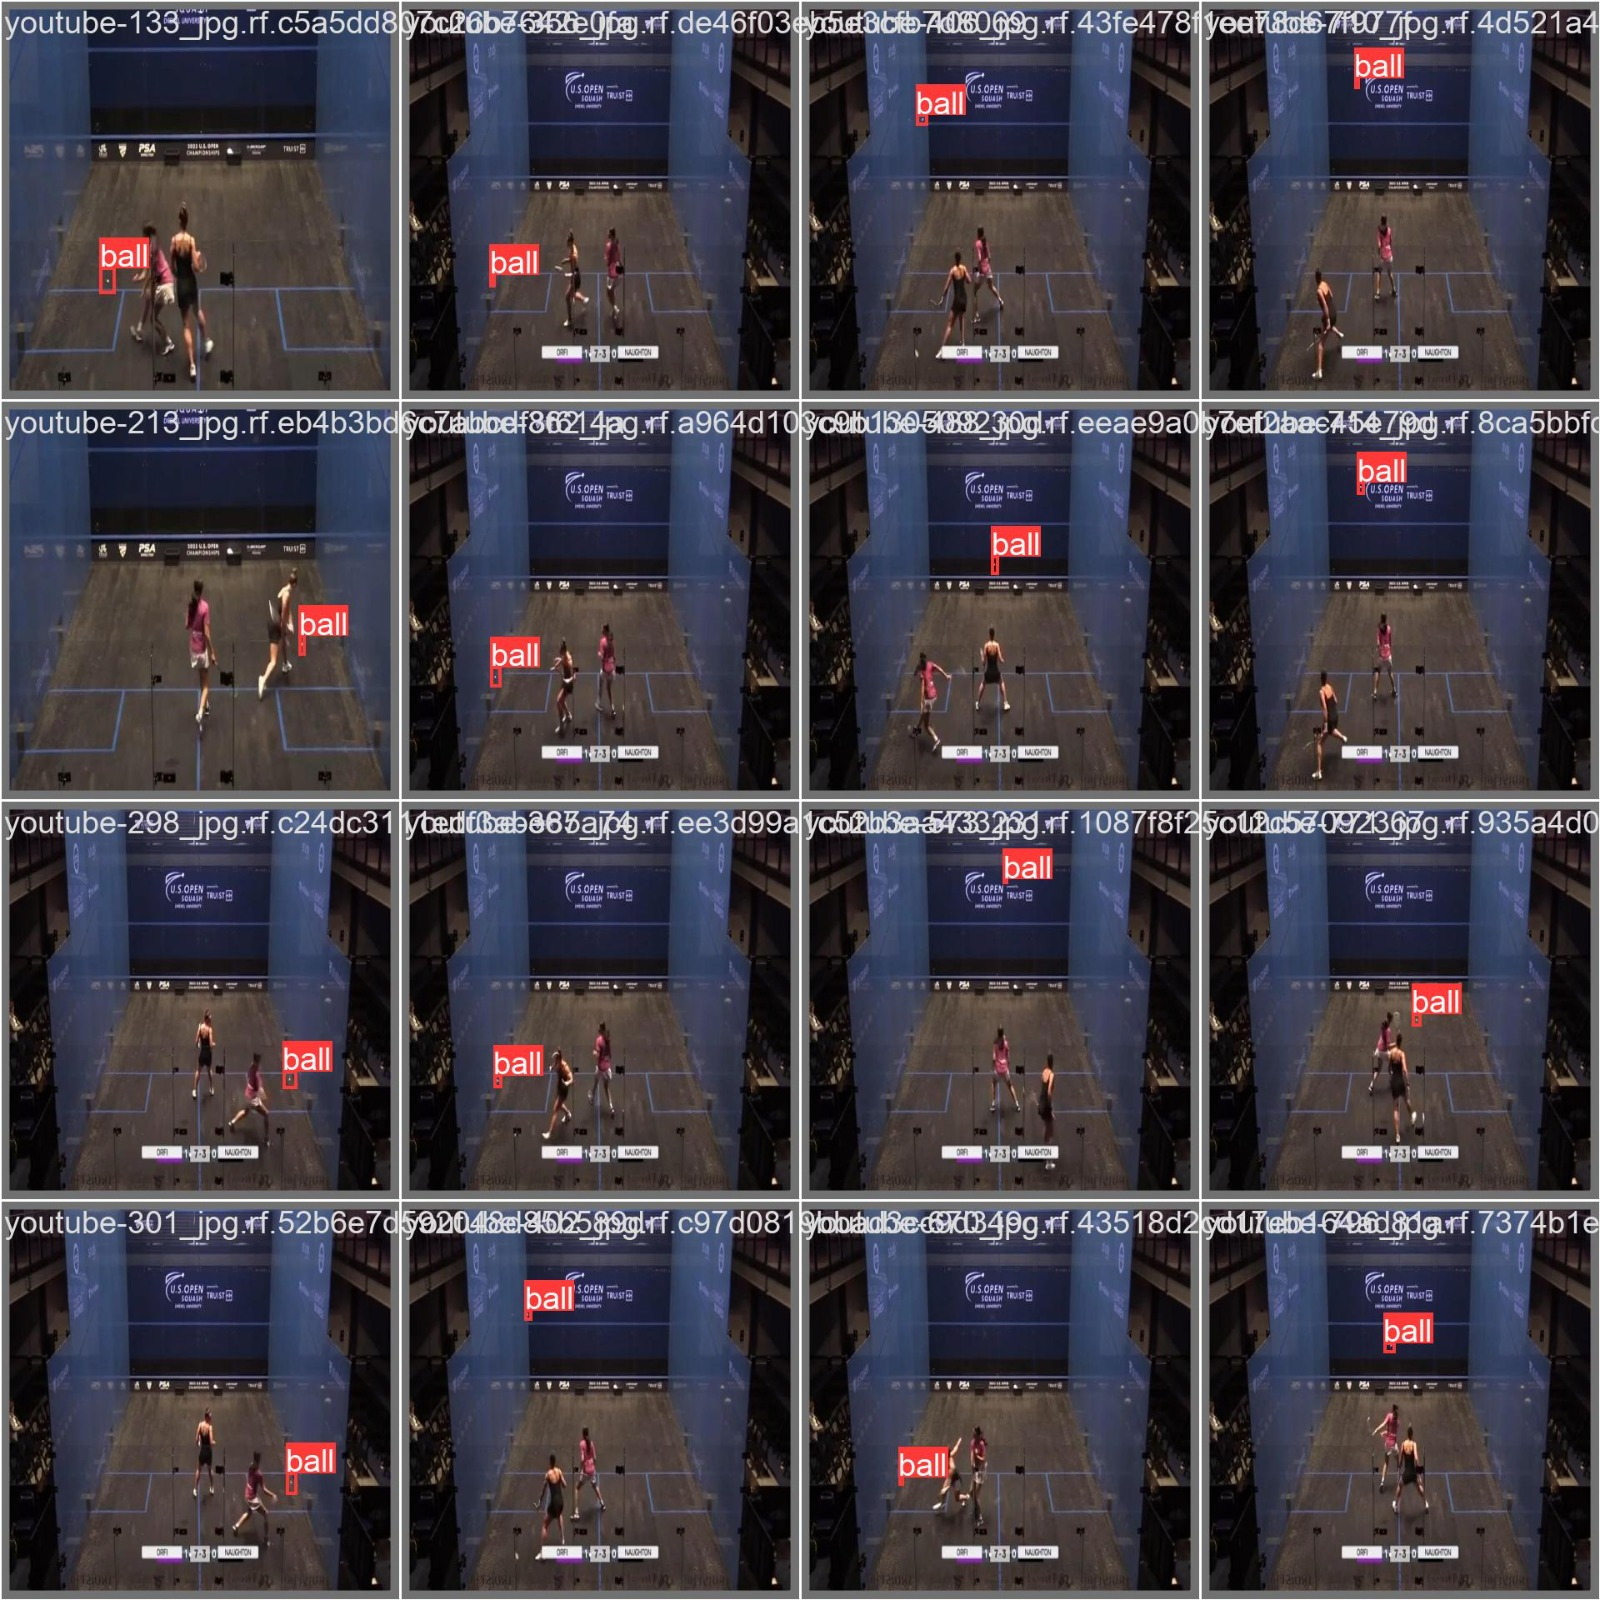
\includegraphics[width=1\linewidth]{figures/ball tracking output.jpg}
        \caption{Ball Tracking Output}
        \label{fig:Ball tracking output}
    \end{figure}

    \begin{figure}[H]
        \centering
        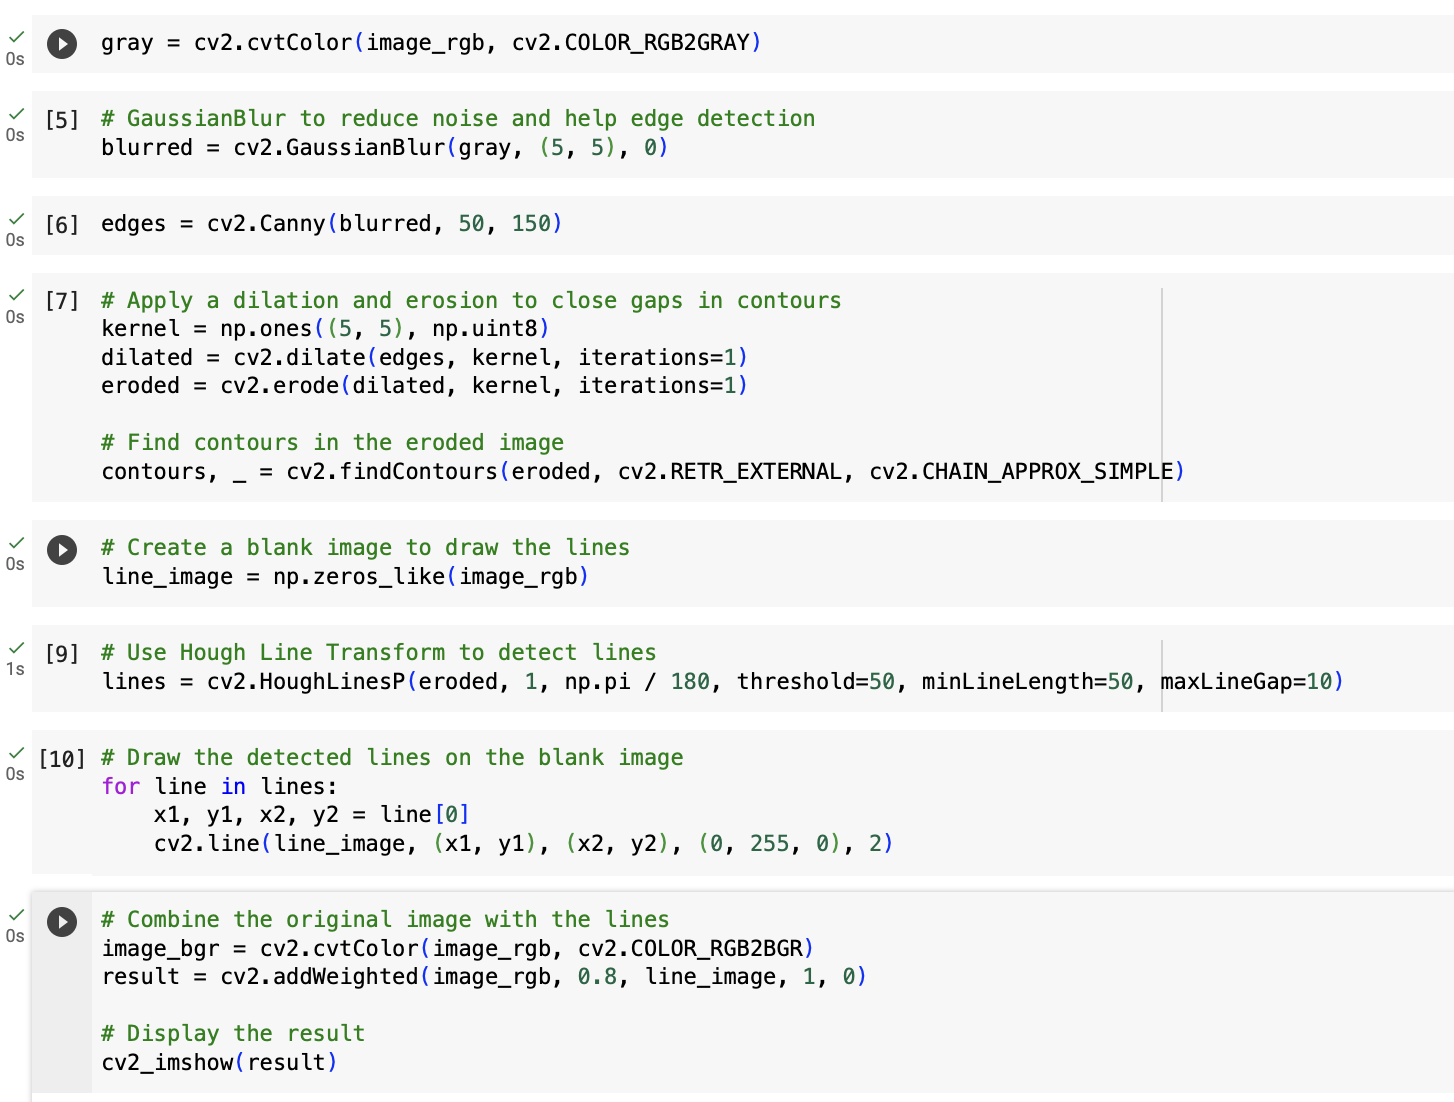
\includegraphics[width=1\linewidth]{figures/Segmentation code.png}
        \caption{Court Segmentation Code}
        \label{fig:Court Segmentation Code}
    \end{figure}

    \begin{figure}[H]
        \centering
        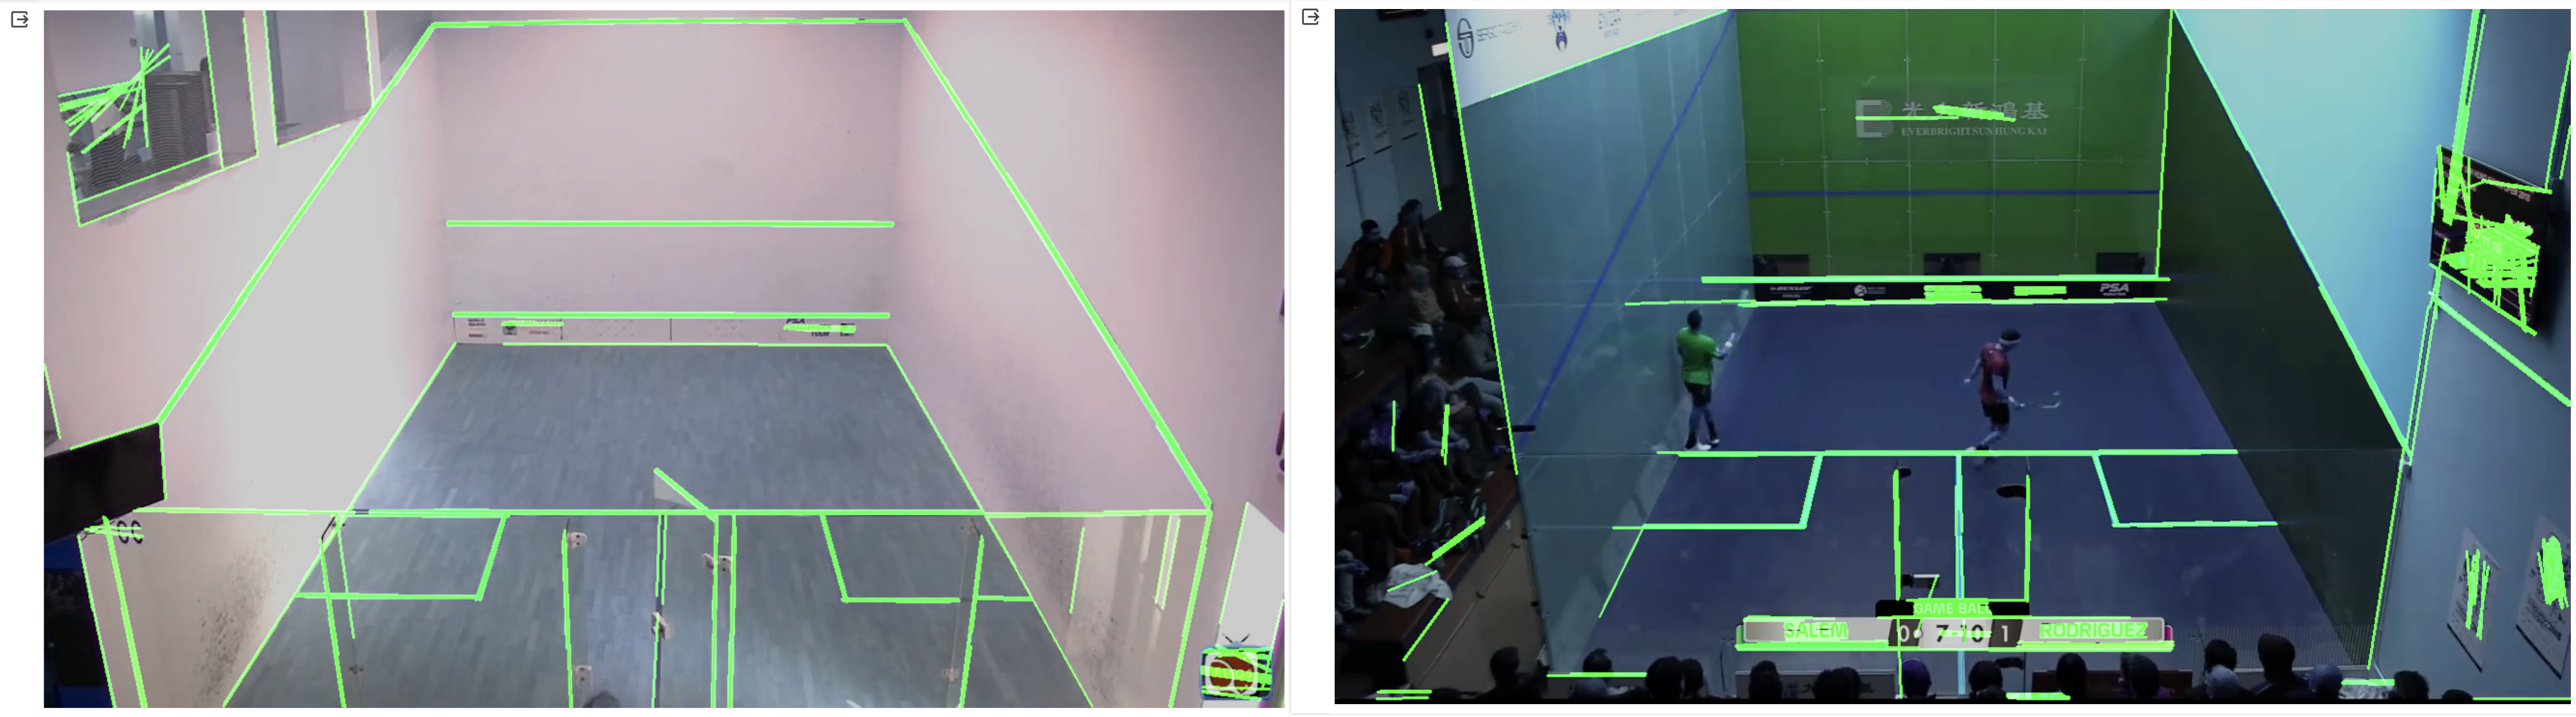
\includegraphics[width=1\linewidth]{figures/Court segmentation Images.jpg}
        \caption{Court Segmentation}
        \label{fig:Court Segmentation image}
    \end{figure}
    

\section{Project Management and Deliverable}
\subsection{Deliverables}
This project will produce a Desktop application used by professional squash organizations ,The system will help referees as it makes the hassle of taking the right decision easier for them. Hence, the team shall deliver not only a functioning Desktop application but also multiple system documentation as well as published papers.

\begin{itemize}
    \item Software proposal document.
    \item Software Requirements Specification (SRS) Document: Describes the nature of the software.
    \item Software Design Description (SDD) Document: Represents the software design.
    \item  Thesis Document: Presents all the research done to deploy the application and its results.
    \item  Research and Academic Papers.
    \item The Desktop Application.
    
\end{itemize}

\subsection{Tasks and Time Plan}
The guideline for the project is as follows:

\begin{figure}[H]
    \centering
    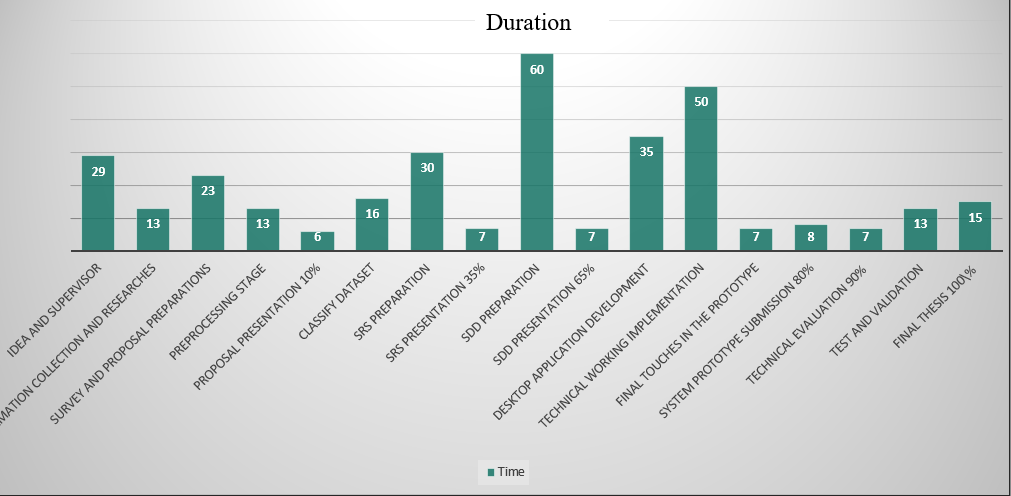
\includegraphics[width=0.95\linewidth]{figures/Time chart.png}
    \label{fig:Time Plan Chart}
\end{figure}

\begin{figure}[H]
    \centering
    \begin{tabular}{|l|l|l|l|l|} 
    \hline 
    \multicolumn{1}{|c|}{\textbf{Tasks}} & \multicolumn{1}{c|}{\textbf{Start Date}} & \multicolumn{1}{c|}{\textbf{End Date}} & \multicolumn{1}{c|}{\textbf{Duration}} & \multicolumn{1}{c|}{\textbf{Team Member}} \\
    \hline
    Idea and Supervisor & 20/8/2023 & 18/09/202 & 29 days & All Team members \\
    \hline
    Information Collection and Researches  & 22/09/2023 & 05/10/2023 & 13 days & All Team members \\
    \hline
    Survey and proposal Preparations & 06/10/2023 & 29/10/2023 & 23 days & All Team Members \\
    \hline
    Preprocessing Stage  & 01/11/2023 & 14/11/2023 & 13 days & All Team Members \\
    \hline
    Proposal Presentation 10\%  & 14/11/2023 & 20/11/2023 & 6 days & All Team Members \\
    \hline
    Classify dataset  & 26/11/2023 & 11/12/2023 & 16 days & All Team Members \\ 
    \hline
    SRS Preparation  & 12/12/2023 & 11/01/2024 & 30 days & All Team Members \\ 
    \hline
    SRS Presentation 35\% & 11/01/2024 & 18/01/2024 & 7 days & All Team Members \\
    \hline
    SDD Preparation & 20/1/2024 & 21/3/2024 & 60 days & All Team Members \\
    \hline
    SDD Presentation 65\%  & 01/3/2024& 25/3/2024 & 7 days& All Team Members \\ 
    \hline
    Desktop Application Development & 08/01/2024& 12/02/2024& 35 days& All Team Members \\ 
    \hline
    Technical Working Implementation & 12/02/2024& 02/04/2024& 50 days & All Team Members \\
    \hline
    Final Touches in The Prototype & 02/04/2024 & 09/04/2024 & 7 days & All Team Members\\ 
    \hline
    System Prototype Submission 80\% & 10/04/2024 & 18/04/2024 & 8 days & All Team Members\\ 
    \hline
    Technical Evaluation 90\% & 26/4/2024 & 03/05/2024 & 7 days & All Team Members\\
    \hline
    Test and Validation & 05/05/2024 & 15/05/2024 & 13 days & All Team Members\\
    \hline
    Final Thesis 100\% & 15/06/2024 & 01/07/2024 & 15 days & All Team Members\\
    \hline
    \end{tabular}
    \caption{Tasks and Time Plan}
    \label{tab:tasks_time_plan}
\end{figure}

\section{Supportive Documents}

\begin{itemize}
    \item Dataset
    \newline
        \begin{enumerate}
    
            \item SQUASHTV youtube channel
            \newline
            In the proposed system, our dataset is scraped from (SQUASHTV youtube channel) which proved a generous amount of rallies as we want. Squash TV is the official live and video-on-demand website of online service exclusively for squash developed by the Professional Squash Association, the most important governing body for the men's and women's professional squash circuit.
        \begin{figure}[H]
            \centering
            
\includegraphics{figures/squashtv_logo.jpg}
            \caption{SQUASHTV Chanel Logo}
            \label{fig:squashtv}
        \end{figure}
        
            \item world squash officiating
            \newline
                WSO is an organization consists of a team of highly skilled and
                trained individuals who play a pivotal role in ensuring fair play.
                The website offers videos of referees' incorrect decisions and their correction.
                
                \begin{figure}[H]
                \centering
                
\includegraphics[width=0.5\linewidth]{figures/wso.jpg}
                \caption{world squash officiating}
                \label{fig:world squash officiating}
                \end{figure}
        \end{enumerate}
    
    \item Survey 
    
    
    A survey had been done to get a wider scope on the need for our project and expand our research. 15 Squash pro players , 2  referees , 1 Coach and 20 regular fans.
    The responses' niches varied from pro players niche, to various watchers including regular fans \& from time to time watchers , coaches and referees. 
    The results indicated how much our respondents were interested in squash and  enthusiastic to see it applied in real matches.
    \end{itemize}
    
    \begin{figure}[H]
    \centering
    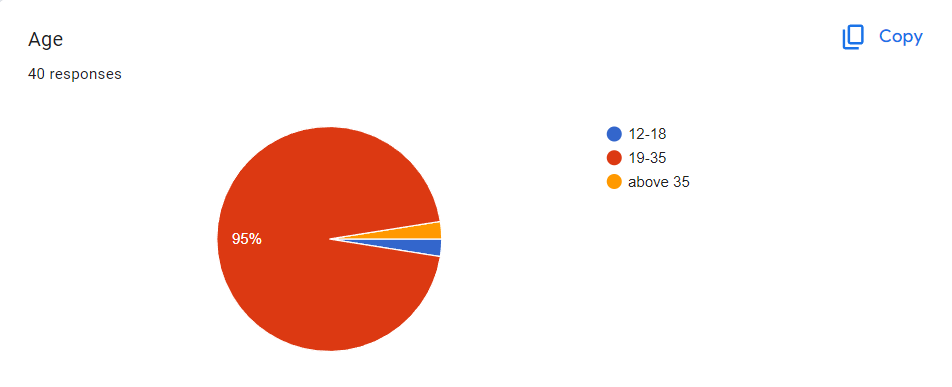
\includegraphics[width=0.7\linewidth]{figures/age.png}
    \label{fig:Question 1}
    \end{figure}
    
    \begin{figure}[H]
    \centering
    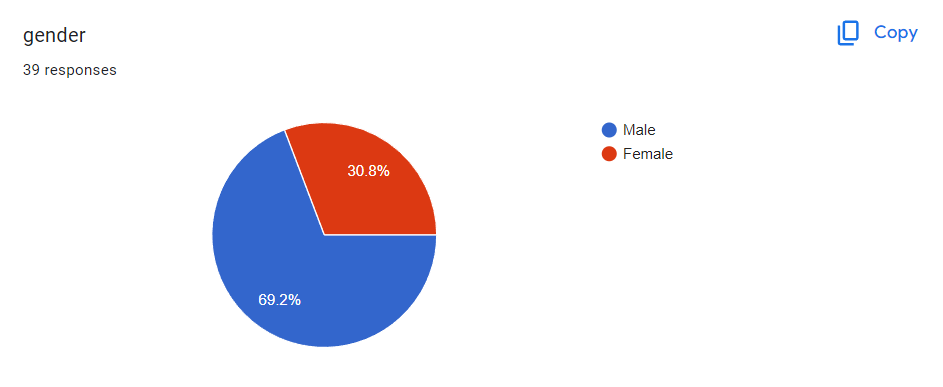
\includegraphics[width=0.7\linewidth]{figures/gender.png}
    \label{fig:Question 2}
    \end{figure}
    
    \begin{figure}[H]
    \centering
    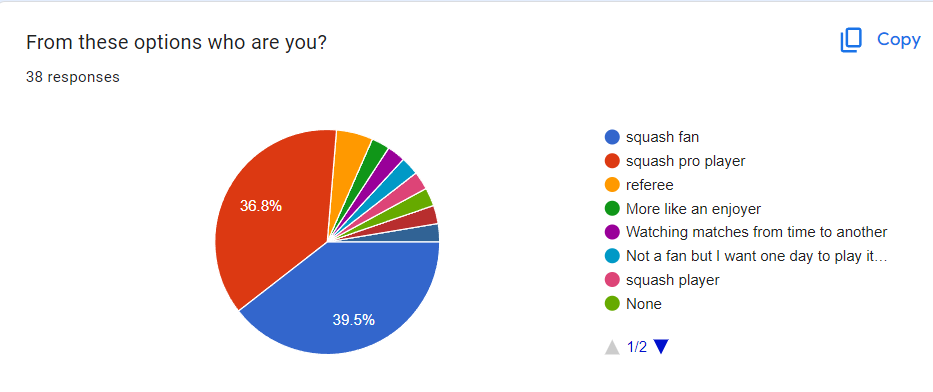
\includegraphics[width=0.7\linewidth]{figures/who are you.png}
    \label{fig:Question 3}
    \end{figure}
    
    \begin{figure}[H]
    \centering
    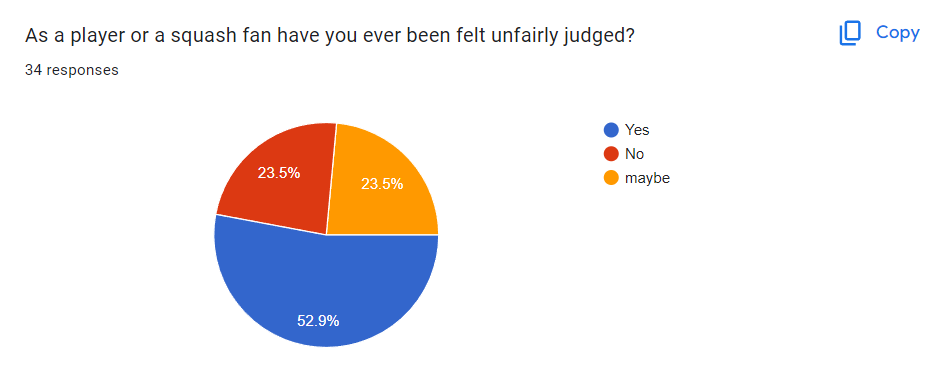
\includegraphics[width=0.7\linewidth]{figures/unfairly judged.png}
    \label{fig:Question 4}
    \end{figure}
    
    \begin{figure}[H]
    \centering
    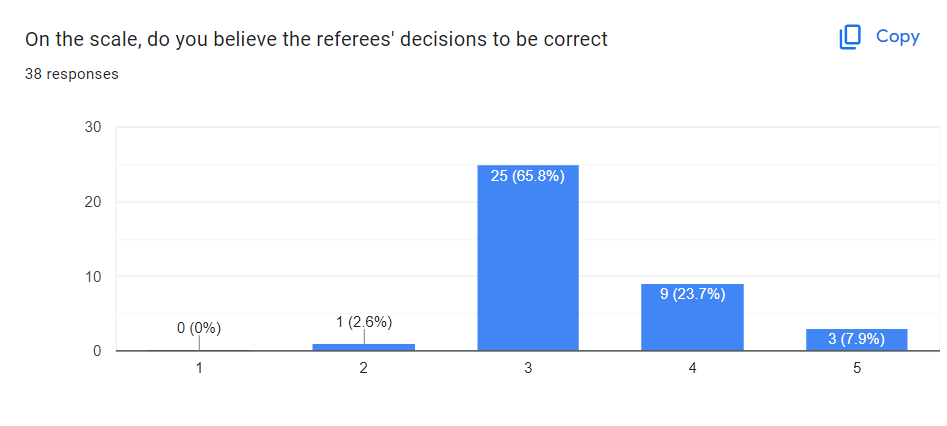
\includegraphics[width=0.7\linewidth]{figures/to be correct.png}
    \label{fig:Question 5}
    \end{figure}
    
    \begin{figure}[H]
    \centering
    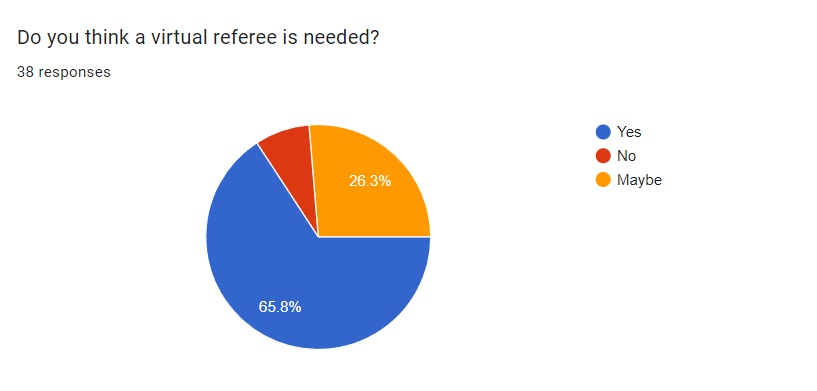
\includegraphics[width=0.7\linewidth]{figures/virtual referee.png}
    \label{fig:Question 6}
    \end{figure}

% \bibliographystyle{alpha}
% \bibliography{sample}
\section {References}
\printbibliography
\end{document}
